\section{Ambiente virtual}
	Para iniciar a modelagem do Parque Virtual foi escolhido um mapa em escala de 
cinza para que sirva de base para a montagem do terreno do ambiente virtual.Para isso 
qualquer editor de imagem pode ser utilizado , no caso do projeto foi utilizado o photoshop,
e a imagem foi tratada e exportada para o formato aceito pelo Unity que é o 'RAW' . Abaixo estão 
as imagens do arquivo do ambiente virtual em escala de cinza e o ambiente virtual que foi gerado.

\begin{figure}[htpb]
 \begin{center}
    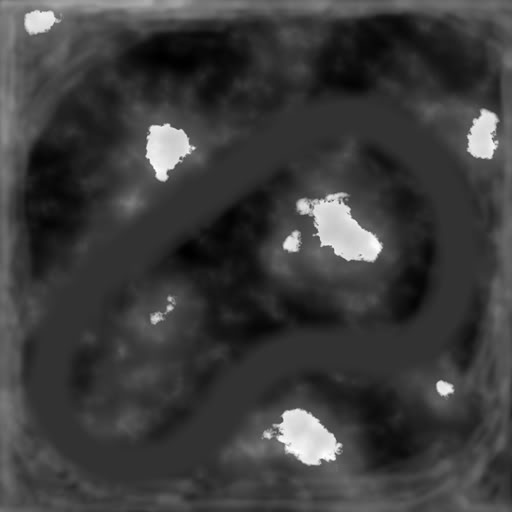
\includegraphics[width=.40\textwidth]{figuras/mapa_escala_de_cinza.jpg}
 \end{center}
  \caption{Mapa do ambiente virtual em escala de cinza}
  \label{fig:core_concurrent}
\end{figure}

\begin{figure}[htpb]
 \begin{center}
    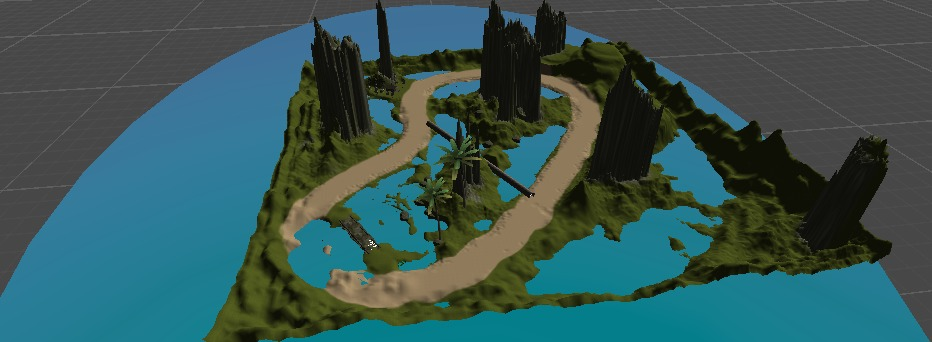
\includegraphics[width=.60\textwidth]{figuras/mapa.png}
 \end{center}
  \caption{Mapa do ambiente virtual gerado e modificado}
  \label{fig:core_concurrent}
\end{figure}

O mapa foi importado para o Unity e foi colocada nele uma base de grama para que
os outros componentes sejam colocadas por cima desta base.Foi feita uma adequação 
do terreno formado pelo mapa de cores para que fosse criada
a ciclovia e na parte mais baixa do mapa foi adicionado água para termos pequenos 
lagos.

Os elementos que estão sendo adicionados no conforme idéias e necessidades encontradas
pela equipe, primeiramente inserimos algumas árvores e vegetações para dar uma visão
de parque ao mapa, inserimos também uma ponte para que o usuário possa passar por um 
ponto de água, está sendo elaborado um túnel para que o usuário possa passar e uma 
cachoeira para ser admirada durante o passeio no ambiente. Para uma melhor visualização 
dos ambiente que estarão no ambiente virtual abaixo estão algumas imagens tiradas do ambiente
 no processo de montagem usando o unity.

\begin{figure}[htpb]
 \begin{center}
    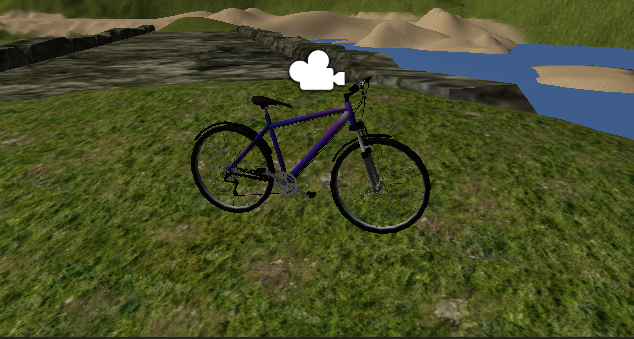
\includegraphics[width=.60\textwidth]{figuras/bicycle.png}
 \end{center}
  \caption{Bicicleta utilizada pelo usuário no ambiente virtual}
  \label{fig:core_concurrent}
\end{figure}

\begin{figure}[htpb]
 \begin{center}
    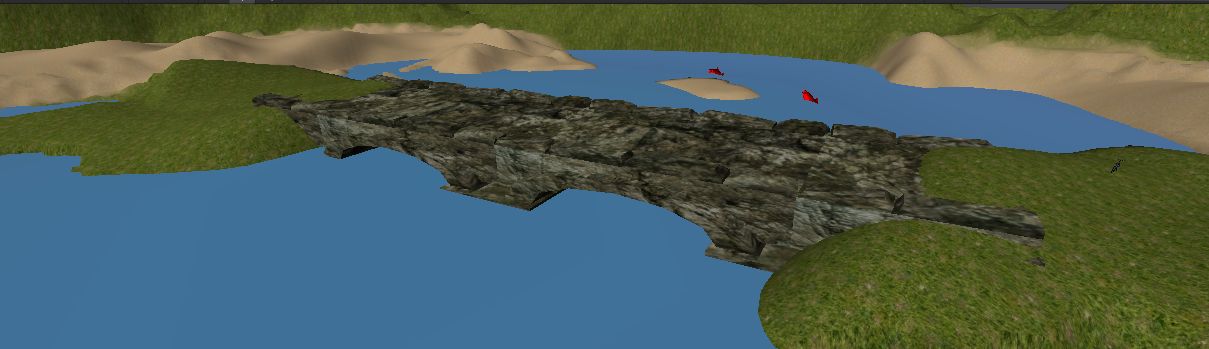
\includegraphics[width=.60\textwidth]{figuras/bridge.png}
 \end{center}
  \caption{Ponte para uma atravessia no lago}
  \label{fig:core_concurrent}
\end{figure}

\begin{figure}[htpb]
 \begin{center}
    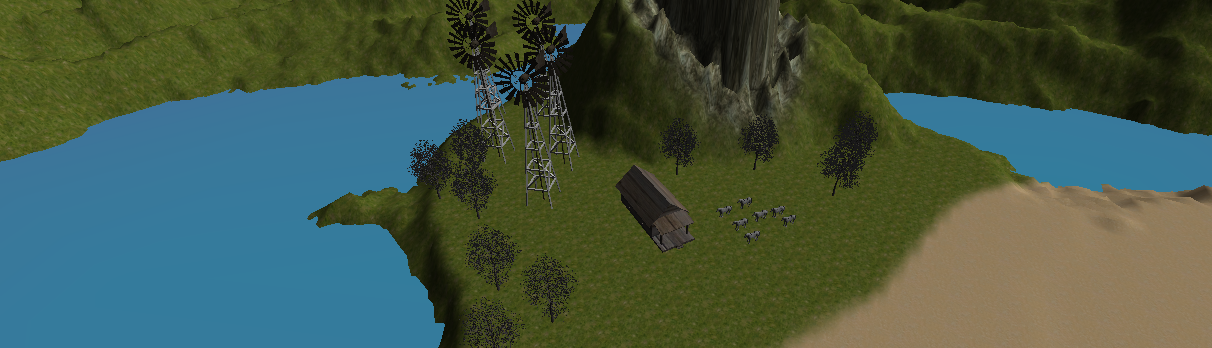
\includegraphics[width=.60\textwidth]{figuras/farm.png}
 \end{center}
  \caption{Fazenda criada em uma área do ambiente virtual}
  \label{fig:core_concurrent}
\end{figure}

\begin{figure}[htpb]
 \begin{center}
    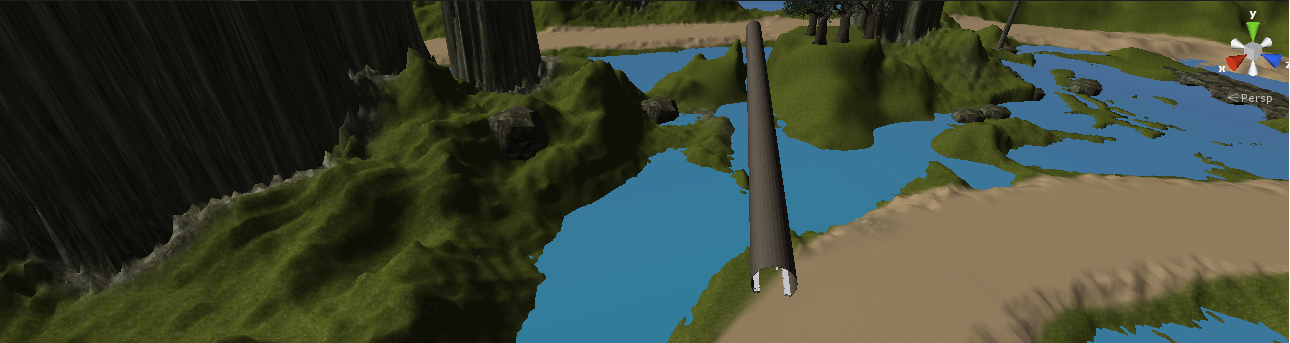
\includegraphics[width=.60\textwidth]{figuras/tunel1.png}
 \end{center}
  \caption{Visão 1 do tunel gerado no ambiente virtual}
  \label{fig:core_concurrent}
\end{figure}

\begin{figure}[htpb]
 \begin{center}
    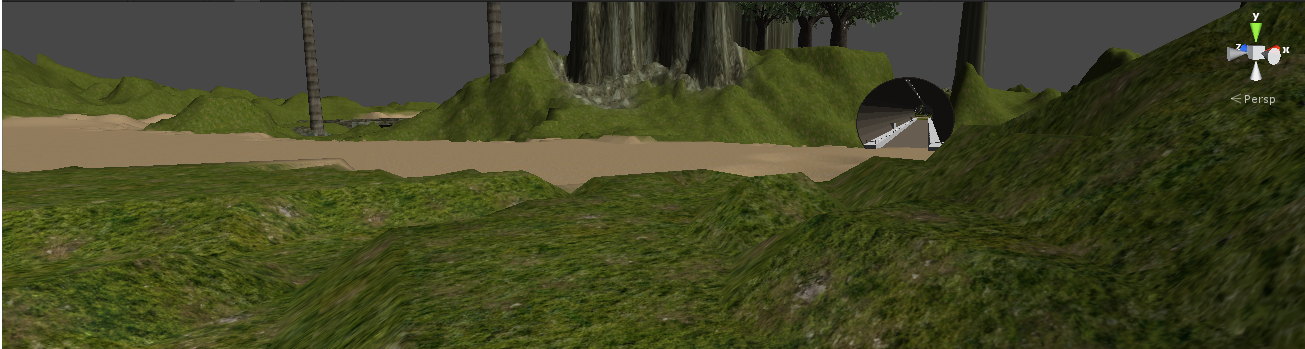
\includegraphics[width=.60\textwidth]{figuras/tunel2.png}
 \end{center}
  \caption{Visão 2 do tunel gerado no ambiente virtual}
  \label{fig:core_concurrent}
\end{figure}

\begin{figure}[htpb]
 \begin{center}
    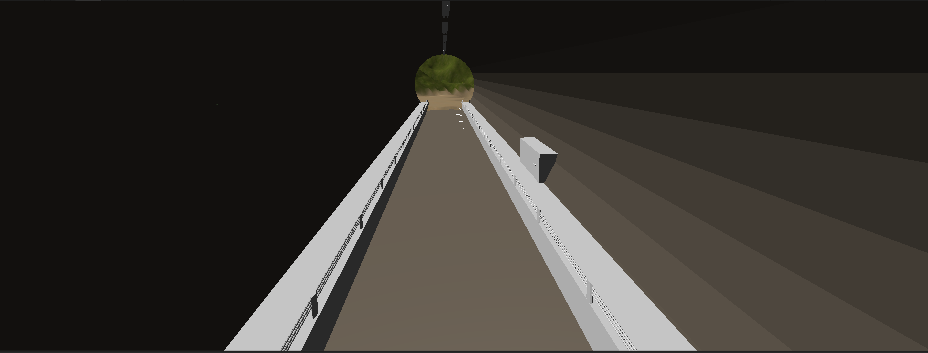
\includegraphics[width=.60\textwidth]{figuras/tunel3.png}
 \end{center}
  \caption{Visão interior do tunel}
  \label{fig:core_concurrent}
\end{figure}

\begin{figure}[htpb]
 \begin{center}
    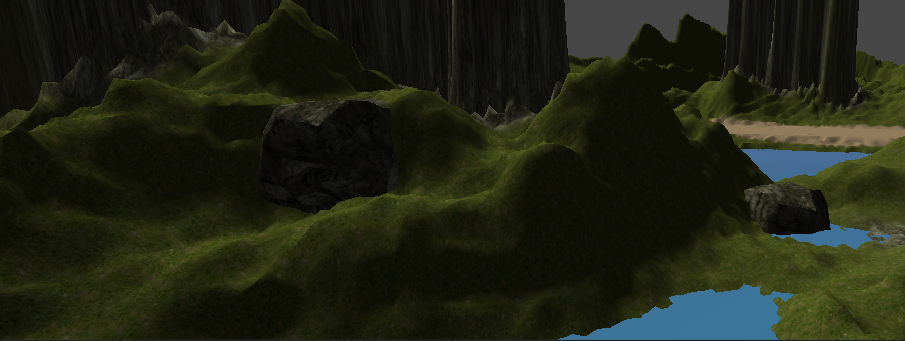
\includegraphics[width=.60\textwidth]{figuras/rock.png}
 \end{center}
  \caption{Visão de algumas pedras para dar mais realizadade ao ambiente}
  \label{fig:core_concurrent}
\end{figure}

\begin{figure}[htpb]
 \begin{center}
    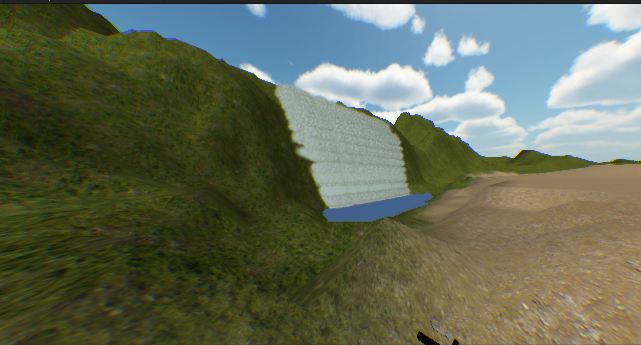
\includegraphics[width=.60\textwidth]{figuras/waterfall.png}
 \end{center}
  \caption{Visão de uma Cachoeira}
  \label{fig:core_concurrent}
\end{figure}

